\documentclass[aspectratio=169,fleqn]{beamer}
\PassOptionsToPackage{english}{babel}
\usepackage{standardslides}

\usepackage{svg}

\usepackage{tikz}
\usepackage{pifont}
\usepackage{listings}
\usepackage{colortbl}
\newlength{\listingframemargin}
\setlength{\listingframemargin}{1em}
\newlength{\listingmargin}
\setlength{\listingmargin}{0.08\textwidth}

\definecolor{codeDarkGray}{gray}{0.2}
\definecolor{codeGray}{gray}{0.4}
\definecolor{codeLightGray}{rgb}{0.94,0.94,0.91}
\definecolor{codeBorder}{rgb}{0.34,0.24,0.21}
\definecolor{MidnightBlue}{rgb}{0.1, 0.1, 0.8}

\lstdefinestyle{standard}{%
  belowcaptionskip=0.5\baselineskip,
  breaklines=true,
  frameround=tttt,
  % frame=false,
  xleftmargin=0em,
  xrightmargin=0em,
  showstringspaces=false,
  showtabs=false,
  % tab=\smash{\rule[-.2\baselineskip]{.4pt}{\baselineskip}\kern.5em},
  basicstyle= \fontfamily{pcr}\selectfont\tiny\bfseries,
  keywordstyle= \bfseries\color{MidnightBlue}, %\color{codeDarkGray},
  commentstyle= \itshape\color{codeGray},
  identifierstyle=\color{codeDarkGray},
  stringstyle=\color{BurntOrange}, %\color{codeDarkGray},
  numberstyle=\tiny\ttfamily,
  % numbers=left,
  numbersep = 1em,
  % stepnumber = 1,
  % captionpos=t,
  tabsize=2,
  % backgroundcolor=\color{codebLightGray},
  rulecolor=\color{codeBorder},
  framexleftmargin=\listingframemargin,
  framexrightmargin=\listingframemargin
}

\newcommand{\inputCodeBlock}[1]{%
  % \begin{mybox}
    \begin{center}
      % \begin{minipage}[c]{0.7\textwidth}
        \lstinputlisting[%
          style = standard,
          language = c++,
          morekeywords={constexpr,noexcept,decltype,size_t,uint32_t,uint64_t,__m256i,__m256,__m256d,__m128i,__m128,__m128d}
        ]{#1}
      % \end{minipage}
    \end{center}
  % \end{mybox}
}

\def\UrlBigBreaks{\do\/\do-\do:}

\setbeamertemplate{background}{
  
\includegraphics[width=\paperwidth,height=\paperheight]{images/background.png}
}

\title{%
  Algorithmical Geometry: Delaunay Triangulation%
}
% \subtitle{Master's Thesis Defense and Presentation}
\author{Markus Pawellek}

\bibliography{references}

\begin{document}

\selectlanguage{english}

{ % all template changes are local to this group.
  \setbeamertemplate{navigation symbols}{}
  \begin{frame}<article:0>[plain]
    \begin{tikzpicture}[remember picture,overlay]
      \node[at=(current page.center)] {
        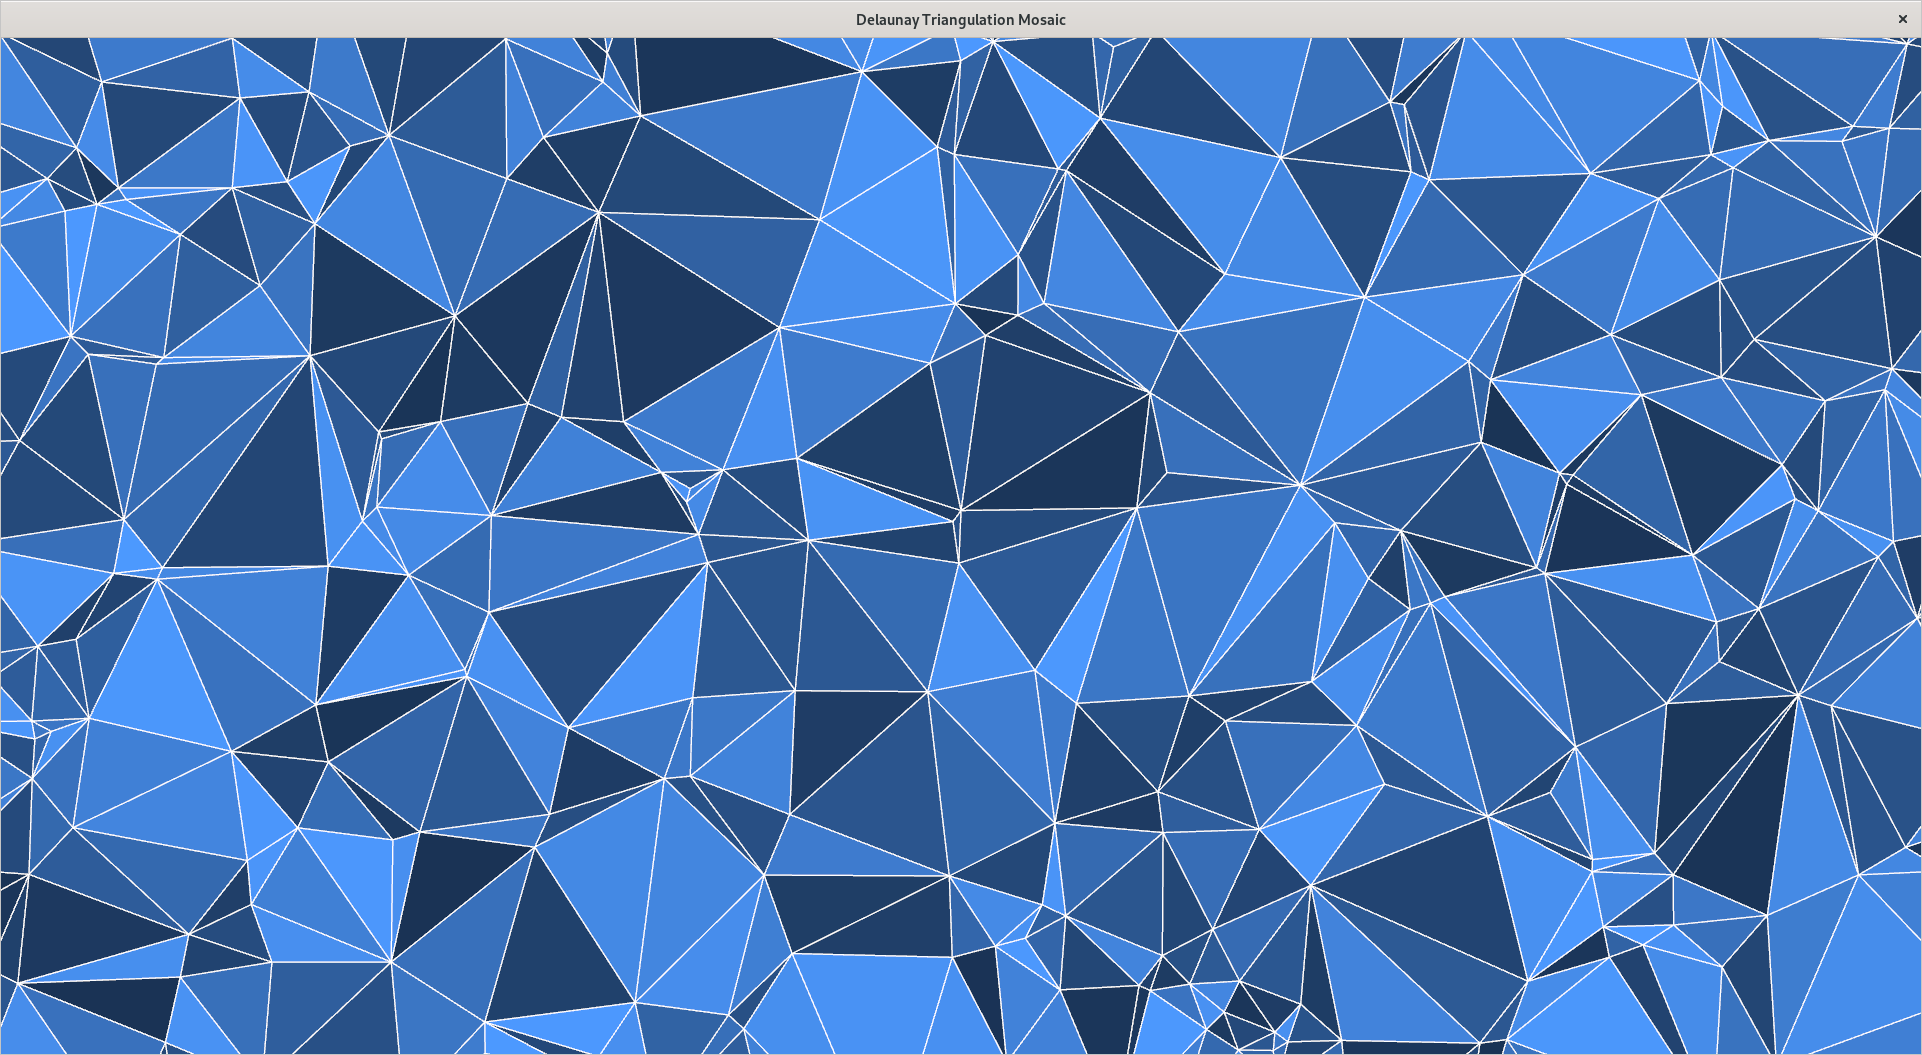
\includegraphics[keepaspectratio,
                         width=1.2\paperwidth,
                         height=\paperheight]{images/banner.png}
      };
    \end{tikzpicture}
  \end{frame}
}

\frame{\titlepage}
\begin{frame}{Outline}
  \footnotesize
  \hfill\parbox[t][7cm][l]{0.9\textwidth}{\tableofcontents}
\end{frame}

\section{Introduction}
  \begin{frame}{Introduction}
    % !!!Here should be an image of a wireframe for a mesh or a 3D grid for FEM simulation.
    % \bigskip
    \begin{minipage}[c]{0.49\textwidth}
      \begin{figure}
        \centering
        \includesvg[width=0.9\textwidth]{images/mesh-generation.svg}
      \end{figure}
      {%
        \fontsize{4}{5}\selectfont%
        *\url{https://upload.wikimedia.org/wikipedia/commons/b/b8/Approx-3tori.svg}, December 29, 2021%
      }
    \end{minipage}
    \hfill
    \begin{minipage}[c]{0.45\textwidth}
      \pause
      Educational Problems:
      \begin{itemize}
        \pause
        \item Many Resources
        \pause
        \item Duality to Voronoi Diagrams
        \pause
        \item%
          Multiple Algorithm Types: \\
          Incremental, Sweepline, Divide-and-Conquer
        \pause
        \item Varying Data Structures
      \end{itemize}
    \end{minipage}
  \end{frame}

  \begin{frame}{Introduction: Previous Work}
    \small
    \onslide<+->
    \begin{description}
      % This custom command does not work...
      % \newcommand\mycommand[1]{\item[\autocite{#1}] \citeauthor{#1}, \citetitle{#1}, \citeyear{#1}}
      \item<+->[\citeyear{lee1980}] \citeauthor{lee1980}, \citetitle{lee1980}
      \item<+->[\citeyear{guibas1985}] \textbf<7>{\citeauthor{guibas1985}, \citetitle{guibas1985}}
      \item<+->[\citeyear{dwyer1987}] \citeauthor{dwyer1987}, \citetitle{dwyer1987}
      \item<+->[\citeyear{shewchuk1996}] \citeauthor{shewchuk1996}, \citetitle{shewchuk1996}
      \item<+->[\citeyear{fuetterling2014}] \citeauthor{fuetterling2014}, \citetitle{fuetterling2014}
    \end{description}
  \end{frame}

\section{Mathematical Preliminaries}
  \begin{frame}{Mathematical Preliminaries: Triangle and Circumcircle}
    % Definition of a triangle can be difficult.
    % Hence, we use and indirect approach.
    % \onslide<+->
    \begin{minipage}[c]{0.45\textwidth}
      \textbf{Triangle} \\
      $A, B, C \in \setReal^2$ affinely independent \\
      define vertices of a triangle.

      \bigskip

      \pause
      \textbf{Circumcircle}\\
      Circle that intersects with \\
      all vertices of the triangle.
    \end{minipage}
    \hfill
    \begin{minipage}[c]{0.49\textwidth}
      \centering
      \onslide<1->
      \only<1>{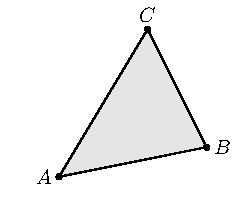
\includegraphics[width=0.9\textwidth]{figures/triangle.pdf}}%
      \only<2>{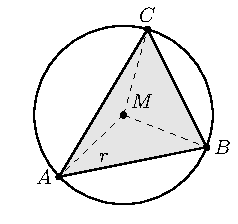
\includegraphics[width=0.9\textwidth]{figures/triangle-circumcirle.pdf}}
    \end{minipage}
  \end{frame}

  \begin{frame}{Mathematical Preliminaries: %
    \only<1>{Point Set}%
    \only<2>{Triangulation}%
    \only<3-5>{Delaunay Triangulation}%
  }
    \begin{minipage}[c]{0.45\textwidth}
      \onslide<+->
      \textbf{Point Set}\\
      $\mathscr{V}\subset\setReal^2$ finite, $\#\mathscr{V}\geq 3$, \\
      affinely span $\setReal^2$

      \bigskip

      \onslide<+->
      \textbf{Triangulation}\\
      Planar straight-line graph over $\mathscr{V}$ \\
      such that its edges form a maximal subset of non-crossing edges.

      \bigskip

      \onslide<+->
      \textbf{Delaunay Triangulation}\\
      Circumcircle of any triangle \\
      contains no other points of $\mathscr{V}$.
    \end{minipage}
    \hfill
    \begin{minipage}[c]{0.49\textwidth}
      \centering
      \onslide<1->
      \only<1>{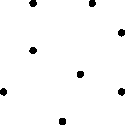
\includegraphics[width=\textwidth]{figures/point-set.pdf}}%
      \only<2>{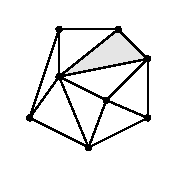
\includegraphics[width=\textwidth]{figures/triangulation.pdf}}%
      \only<3>{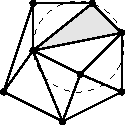
\includegraphics[width=\textwidth]{figures/triangulation-circumcircle.pdf}}%
      \only<4>{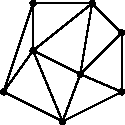
\includegraphics[width=\textwidth]{figures/delaunay-triangulation.pdf}}%
      \only<5>{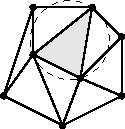
\includegraphics[width=\textwidth]{figures/delaunay-triangulation-circumcircle.pdf}}%
    \end{minipage}
  \end{frame}

  \begin{frame}{Mathematical Preliminaries: Properties}
    \begin{figure}
      \center
      \onslide<1->
      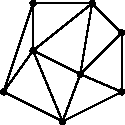
\includegraphics[scale=1.3]{figures/delaunay-triangulation.pdf}
      \onslide<3->
      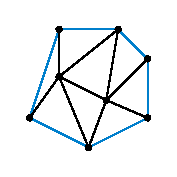
\includegraphics[scale=1.3]{figures/delaunay-triangulation-convex-hull.pdf}
      \onslide<4->
      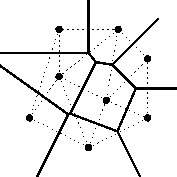
\includegraphics[scale=1.3]{figures/delaunay-triangulation-voronoi.pdf}
    \end{figure}
    \begin{itemize}
      \onslide<2->
      \item Optimality: maximization of the minimum angle of all angles
      \onslide<3->
      \item Convex hull is contained
      \onslide<4->
      \item Voronoi diagram is the dual
    \end{itemize}
  \end{frame}

  \begin{frame}{Mathematical Preliminaries: Properties of Delaunay Triangulation}
    \begin{itemize}
      \item Duality to Voronoi Diagram (also useful for proofs)
      \item always exists -> proof
      \item If no points are cocircular, unique -> proof
      \item optimality: maximization of the minimum angle of all angles -> proof, reason why delaunay is good
      \item boundary is convex hull
    \end{itemize}
  \end{frame}

\section{Geometric Primitives}
  \begin{frame}{Geometric Primitives: Counterclockwise}
    \begin{minipage}[c]{0.4\textwidth}
      %\begin{figure}
        \centering
        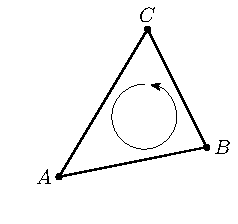
\includegraphics{figures/triangle-counterclockwise.pdf}
      %\end{figure}
    \end{minipage}
    \hfill
    $\longleftrightarrow$
    \hfill
    \begin{minipage}[c]{0.4\textwidth}
      %\begin{figure}
        \centering
        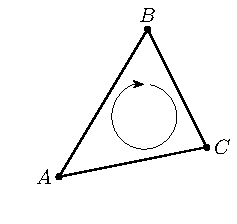
\includegraphics{figures/triangle-clockwise.pdf}
      %\end{figure}
    \end{minipage}

    Counterclockwise Order
    \pause
    $\quad\iff\quad$ $C$ is left of $\overline{AB}$

    \bigskip

    \pause
    \begin{mybox}
    \[
      0 <
      \begin{vmatrix}
        A_x & A_y & 1 \\
        B_x & B_y & 1 \\
        C_x & C_y & 1 \\
      \end{vmatrix}
      \pause
      =
      \begin{vmatrix}
        B_x - A_x & B_y - A_y \\
        C_x - A_x & C_y - A_y \\
      \end{vmatrix}
      \pause
      =
      \det
      \begin{pmatrix}
        B-A && C-A
      \end{pmatrix}
    \]
    \end{mybox}
  \end{frame}

  \begin{frame}{Geometric Primitives: Inside Circumcircle}
    \pause
    \begin{minipage}[c]{0.49\textwidth}
      \begin{mybox}
      \[
        0 <
        \begin{vmatrix}
          A_x & A_y & A_x^2 + A_y^2 & 1 \\
          B_x & B_y & B_x^2 + B_y^2 & 1 \\
          C_x & C_y & C_x^2 + C_y^2 & 1 \\
          D_x & D_y & D_x^2 + D_y^2 & 1 \\
        \end{vmatrix}
      \]
      %\[
      %  =
      %  \scalarProduct{x}{\mathrm{adj}\begin{pmatrix}u & v \end{pmatrix}^\mathrm{T} \begin{pmatrix}\norm{u}^2 \\ \norm{v}^2 \end{pmatrix}} - \det\begin{pmatrix}u & v \end{pmatrix}\norm{x}^2
      %\]
      \end{mybox}
    \end{minipage}
    \hfill
    \begin{minipage}[c]{0.49\textwidth}
      \center
      \onslide<1->
      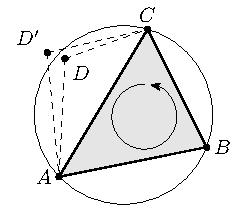
\includegraphics[width=0.9\textwidth]{figures/inside-circumcircle.pdf}
    \end{minipage}
  \end{frame}

\section{Data Structure}
  \begin{frame}{Data Structure: Quad-Edge}
    \begin{minipage}[c]{0.49\textwidth}
      Edge-Based List-Like Data Structure:
      \onslide<+->
      \begin{itemize}
        \item<+-> Directed edges for vertices
        \item<+-> Pointer to ccw. next directed edge with same origin vertex
        \item<+-> Directed dual edges for adjacent faces
        \item<+-> Pointer to ccw. next directed dual edge with same origin face
      \end{itemize}
    \end{minipage}
    \hfill
    \begin{minipage}[c]{0.49\textwidth}
      \center
      \only<1>{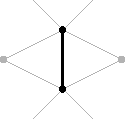
\includegraphics[width=0.9\textwidth]{figures/quad-edge-empty.pdf}}%
      \only<2-3>{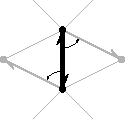
\includegraphics[width=0.9\textwidth]{figures/quad-edge.pdf}}%
      \only<4-5>{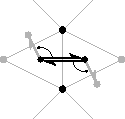
\includegraphics[width=0.9\textwidth]{figures/quad-edge-dual.pdf}}%
      \only<6->{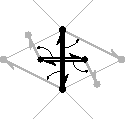
\includegraphics[width=0.9\textwidth]{figures/quad-edge-both.pdf}}%
    \end{minipage}
  \end{frame}

  \begin{frame}{Data Structure: Quad-Edge Implementation}
    \begin{minipage}[c]{0.49\textwidth}
      %\onslide<1>
      \only<1>{%
        \begin{figure}
          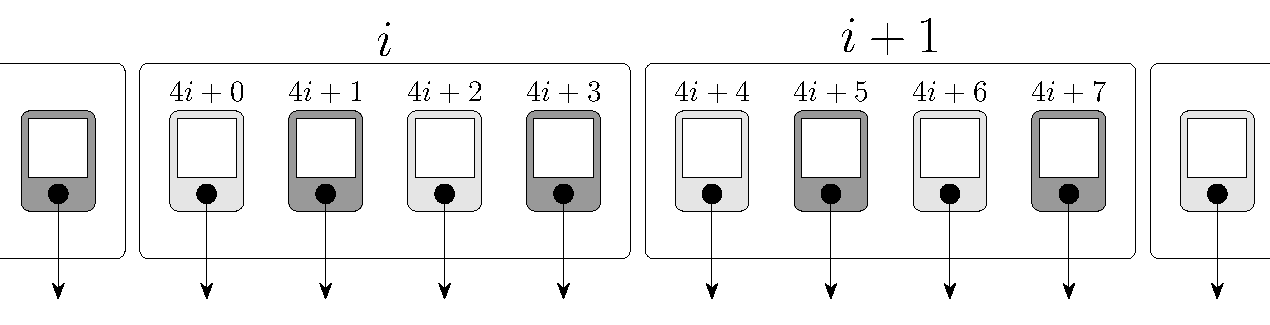
\includegraphics[width=\textwidth]{figures/quad-edge-struct.pdf}
        \end{figure}%
        \begin{mybox}
          \center
          \vspace{-1em}
          \inputCodeBlock{listings/quad-edge-algebra.cpp}
        \end{mybox}%
      }%
      %\onslide<2>
      \only<2>{%
        %\begin{mybox}
        %  \inputCodeBlock{listings/quad-edge-algebra-operations.cpp}
        %\end{mybox}}%
        \begin{figure}
          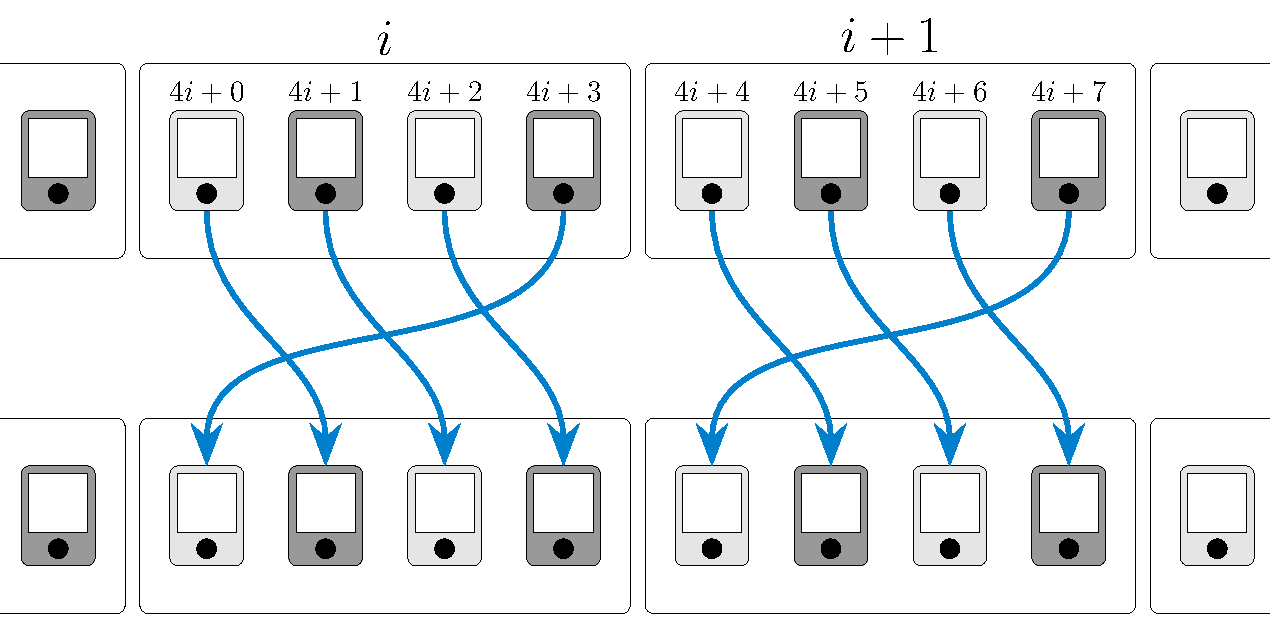
\includegraphics[width=\textwidth]{figures/quad-edge-struct-rot.pdf}
        \end{figure}%
        \begin{mybox}
          \[
            \function{\mathrm{rot}}{\setNatural_0}{\setNatural_0}
          \]
          \[
            \mathrm{rot}(x) = 4 \cdot \floorBrackets{\frac{x}{4}} + (x+1 \mod 4)
          \]
        \end{mybox}%
      }%
    \end{minipage}
    \hfill
    \begin{minipage}[c]{0.49\textwidth}
      \center
      \only<1>{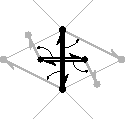
\includegraphics[width=0.9\textwidth]{figures/quad-edge-both.pdf}}%
      \only<2>{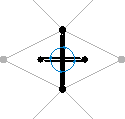
\includegraphics[width=0.9\textwidth]{figures/quad-edge-rot.pdf}}%
    \end{minipage}
  \end{frame}

  \begin{frame}{Data Structure: Quad-Edge Functions}
    \center
    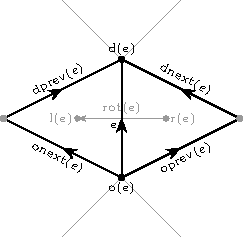
\includegraphics[width=0.49\textwidth]{figures/quad-edge-vertex-functions.pdf}
    \hfill
    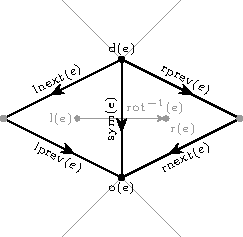
\includegraphics[width=0.49\textwidth]{figures/quad-edge-face-functions.pdf}
  \end{frame}

  \begin{frame}{Data Structure: Quad-Edge Operations}
    \begin{itemize}
      \item edge functions
      \item create edge
      \item splice
      \item connect
      \item delete edge
    \end{itemize}
  \end{frame}

\section{Algorithm}
  \begin{frame}{Algorithm: Overview}
    \begin{enumerate}
      \item Sort points by increasing $x$ coordinate
    \end{enumerate}
    \begin{enumerate}
      \item If number of points is less than four, create an edge or a triangle.
      \item Separate points into left and right half
      \item Compute the lower common tangent and make it a cross edge
      \item Merge Loop to insert crossing edges until upper tangent is reached
      \item Return left and right convex hull edge
    \end{enumerate}
    \begin{enumerate}
      \item Remove edges from left partition that fail circle test
      \item Remove edges from right partition that fail circle test
      \item Check for upper tangent
      \item Insert crossing edge by using circle test
    \end{enumerate}
  \end{frame}

\section{Implementation}
  \begin{frame}{Implementation}
    \begin{itemize}
      \item Geometric Primitives need exact computation and therefore arbitrary precision
    \end{itemize}
  \end{frame}

\section{Applications}

\section{Conclusions}

\begin{frame}
  \vfill
  \centering
  \begin{beamercolorbox}[sep=8pt,center,shadow=true,rounded=true]{title}
    \usebeamerfont{title}%
    Thank you for Your Attention!%
    \par%
  \end{beamercolorbox}
  \vfill
\end{frame}

\begin{frame}
  \frametitle{References}
  % \tiny
  \AtNextBibliography{\tiny}
  \begin{multicols}{2}
    \nocite{*}
    \printbibliography
  \end{multicols}
\end{frame}

\end{document}
